\documentclass[12pt,utf8,notheorems,compress,t]{beamer}
\usepackage{etex}

\usepackage[english]{babel}

\usepackage{mathtools}
\usepackage{booktabs}
\usepackage{array}
\usepackage{ragged2e}
\usepackage{multicol}
\usepackage{tabto}
\usepackage{xstring}
\usepackage{soul}\setul{0.3ex}{}
\usepackage[all]{xy}
\xyoption{rotate}
\usepackage{tikz}
\usetikzlibrary{calc,shapes.callouts,shapes.arrows,patterns}
\hypersetup{colorlinks=true}
\usepackage{multimedia}
\newcommand{\video}[2]{\movie[width=#2,height=#2,autostart,loop,poster]{}{#1}}
\hypersetup{colorlinks=false}

\usepackage{pifont}
\newcommand{\cmark}{\ding{51}}
\newcommand{\xmark}{\ding{55}}

\graphicspath{{images/}}

\usepackage[protrusion=true,expansion=true]{microtype}

\setlength\parskip{\medskipamount}
\setlength\parindent{0pt}

\title{Without loss of generality, any reduced ring is a field}
\author{Ingo Blechschmidt}
\date{April 11th, 2018}

\useinnertheme[shadow=true]{rounded}
\useoutertheme{split}
\usecolortheme{orchid}
\usecolortheme{whale}
\setbeamerfont{block title}{size={}}

\useinnertheme{rectangles}

\usecolortheme{seahorse}
\definecolor{mypurple}{RGB}{150,0,255}
\setbeamercolor{structure}{fg=mypurple}
\definecolor{myred}{RGB}{150,0,0}
\setbeamercolor*{title}{bg=myred,fg=white}
\setbeamercolor*{titlelike}{bg=myred,fg=white}

\usefonttheme{serif}
\usepackage[T1]{fontenc}
\usepackage{libertine}

\newcommand{\A}{\mathcal{A}}
\renewcommand{\AA}{\mathbb{A}}
\newcommand{\CC}{\mathbb{C}}
\newcommand{\E}{\mathcal{E}}
\newcommand{\F}{\mathcal{F}}
\renewcommand{\G}{\mathcal{G}}
\newcommand{\GG}{\mathbb{G}}
\renewcommand{\O}{\mathcal{O}}
\newcommand{\K}{\mathcal{K}}
\newcommand{\NN}{\mathbb{N}}
\newcommand{\RR}{\mathbb{R}}
\newcommand{\TT}{\mathbb{T}}
\newcommand{\PP}{\mathbb{P}}
\newcommand{\ZZ}{\mathbb{Z}}
\renewcommand{\P}{\mathcal{P}}
\newcommand{\aaa}{\mathfrak{a}}
\newcommand{\ppp}{\mathfrak{p}}
\newcommand{\mmm}{\mathfrak{m}}
\newcommand{\defeq}{\vcentcolon=}
\newcommand{\defeqv}{\vcentcolon\equiv}
\newcommand{\Sh}{\mathrm{Sh}}
\newcommand{\GL}{\mathrm{GL}}
\newcommand{\Zar}{\mathrm{Zar}}
\newcommand{\op}{\mathrm{op}}
\newcommand{\Set}{\mathrm{Set}}
\newcommand{\Eff}{\mathrm{Ef{}f}}
\newcommand{\Sch}{\mathrm{Sch}}
\newcommand{\Aff}{\mathrm{Aff}}
\newcommand{\LRS}{\mathrm{LRS}}
\newcommand{\Hom}{\mathrm{Hom}}
\newcommand{\Spec}{\mathrm{Spec}}
\newcommand{\lra}{\longrightarrow}
\newcommand{\RelSpec}{\operatorname{Spec}}
\renewcommand{\_}{\mathpunct{.}}
\newcommand{\?}{\,{:}\,}
\newcommand{\speak}[1]{\ulcorner\text{\textnormal{#1}}\urcorner}
\newcommand{\ull}[1]{\underline{#1}}
\newcommand{\affl}{\ensuremath{{\ull{\AA}^1}}}
\newcommand{\Ll}{\vcentcolon\!\Longleftrightarrow}
\newcommand{\inv}{inv.\@}
\newcommand{\seq}{\vdash_{\!\!\!\vec x}}

\setbeamertemplate{blocks}[rounded][shadow=false]

\newcommand{\fmini}[2]{\framebox{\begin{minipage}{#1}#2\end{minipage}}}
\makeatletter
\def\underunbrace#1{\mathop{\vtop{\m@th\ialign{##\crcr
      $\hfil\displaystyle{#1}\hfil$\crcr\noalign{\kern3\p@\nointerlineskip}
      \crcr\noalign{\kern3\p@}}}}\limits}
\def\overunbrace#1{\mathop{\vbox{\m@th\ialign{##\crcr\noalign{\kern3\p@}
      \crcr\noalign{\kern3\p@\nointerlineskip}
      $\hfil\displaystyle{#1}\hfil$\crcr}}}\limits}
\makeatother

\newenvironment{changemargin}[2]{%
  \begin{list}{}{%
    \setlength{\topsep}{0pt}%
    \setlength{\leftmargin}{#1}%
    \setlength{\rightmargin}{#2}%
    \setlength{\listparindent}{\parindent}%
    \setlength{\itemindent}{\parindent}%
    \setlength{\parsep}{\parskip}%
  }%
  \item[]}{\end{list}}

\newcommand{\pointthis}[2]{%
  \tikz[remember picture,baseline]{\node[anchor=base,inner sep=0,outer sep=0]%
    (#1) {#1};\node[overlay,rectangle callout,%
    callout relative pointer={(0.3cm,1.0cm)},fill=blue!20] at ($(#1.north)+(-0.1cm,-1.6cm)$) {#2};}%
}%

\newcommand{\hcancel}[5]{%
  \tikz[baseline=(tocancel.base)]{
    \node[inner sep=0pt,outer sep=0pt] (tocancel) {#1};
    \draw[red, line width=0.4mm] ($(tocancel.south west)+(#2,#3)$) -- ($(tocancel.north east)+(#4,#5)$);
  }%
}
% Adapted from https://latex.org/forum/viewtopic.php?t=2251 (Stefan Kottwitz)
\newenvironment<>{varblock}[2]{\begin{varblockextra}{#1}{#2}{}}{\end{varblockextra}}
\newenvironment<>{varblockextra}[3]{
  \begin{center}
    \begin{minipage}{#1}
      \begin{actionenv}#4
        {\centering \hil{#2}\par}
	\def\insertblocktitle{}%\centering #2}
        \def\varblockextraend{#3}
	\usebeamertemplate{block begin}}{
        \par
        \usebeamertemplate{block end}
        \varblockextraend
      \end{actionenv}
    \end{minipage}
  \end{center}}

\setbeamertemplate{frametitle}{%
  \vskip0.7em%
  \leavevmode%
  \begin{beamercolorbox}[dp=1ex,center]{}%
      \usebeamercolor[fg]{item}{\textbf{{\Large \insertframetitle}}}
  \end{beamercolorbox}%
}

\setbeamertemplate{navigation symbols}{}

\newcounter{framenumberpreappendix}
\newcommand{\backupstart}{
  \setcounter{framenumberpreappendix}{\value{framenumber}}
}
\newcommand{\backupend}{
  \addtocounter{framenumberpreappendix}{-\value{framenumber}}
  \addtocounter{framenumber}{\value{framenumberpreappendix}} 
}

\setbeamertemplate{footline}{%
  \begin{beamercolorbox}[wd=\paperwidth,ht=2.25ex,dp=1ex,right,rightskip=1mm,leftskip=1mm]{}%
    \hfill
    \insertframenumber\,/\,\inserttotalframenumber
  \end{beamercolorbox}%
  \vskip0pt%
}


\newcommand{\hil}[1]{{\usebeamercolor[fg]{item}{\textbf{#1}}}}

\IfSubStr{\jobname}{\detokenize{nonotes}}{
  \setbeameroption{hide notes}
}{
  \setbeameroption{show notes}
}
\setbeamertemplate{note page}[plain]
\setbeameroption{hide notes}

\begin{document}

\addtocounter{framenumber}{-1}

\begin{frame}[c]
  \centering
  \bigskip
  \bigskip
  \bigskip
  \bigskip

  \large
  \hil{Without loss of generality, \\ any reduced ring is a field.}

  \bigskip

  \emph{\small Interruptions welcome at any point.}

  \bigskip

  \scriptsize
  Ingo Blechschmidt \\
  University of Augsburg
  \bigskip

  Oberseminar Mathematische Logik \\
  Ludwig-Maximilians-Universität München \\
  April 11th, 2018
  \par
\end{frame}


\section{Introduction}

\begin{frame}{Summary}
  \begin{itemize}
    \item For any reduced ring~$A$, there is a semantics with
    \[ A \models \bigl(\forall x\_ \neg(\exists y\_ xy = 1) \Rightarrow x = 0\bigr). \]

    \item This semantics is sound with respect to intuitionistic logic.

    \item \ \\[-1.2em]\mbox{It has uses in classical and constructive commutative
    algebra.}
  \end{itemize}

  \pause
  \vspace*{-0.7em}

  \begin{columns}[t]
    \begin{column}[t]{0.47\textwidth}
      \centering

      \begin{varblock}{\textwidth}{A baby application}
        \justifying
        Let~$M$ be a surjective matrix with more rows than columns over a ring~$A$.
        Then~$A = 0$.
      \end{varblock}

      \scalebox{0.8}{$\begin{pmatrix}
        \cdot & \cdot \\
        \cdot & \cdot \\
        \cdot & \cdot
      \end{pmatrix}$}
    \end{column}

    \begin{column}[t]{0.47\textwidth}
      \centering

      \begin{varblock}{\textwidth}{Generic freeness\phantom{p}}
        \justifying
        Generically, any finitely generated module over a reduced ring is free.
      \end{varblock}
      \vspace*{-0.5em}

      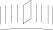
\includegraphics[width=0.6\textwidth]{generic-freeness}
    \end{column}
  \end{columns}
\end{frame}


\section{The semantics}

\subsection[Motivation]{Motivating the semantics}

\begin{frame}{Motivating the semantics}
  \centering
  \begin{varblockextra}{0.8\textwidth}{}{
    \hil{Examples:}\phantom{Non-}\,\! $k,\ k[[X]],\ \CC\{z\},\ \ZZ_{(p)}$ \\[0.2em]
    \hil{Non-examples:} $\ZZ,\ k[X],\ \ZZ/(pq)$
  }
    \justifying
    A ring is \hil{local} iff~$1 \neq 0$ and~$x + y = 1$ implies that~$x$ is
    invertible or~$y$ is invertible.
  \end{varblockextra}

  \begin{varblockextra}{0.8\textwidth}{}{
    Let~$x + y = 1$ in a ring~$A$.
    Then:
    \begin{itemize}
      \item The element $x$ is invertible in~$A[x^{-1}]$.
      \item The element $y$ is invertible in~$A[y^{-1}]$.
    \end{itemize}
  }
    \hil{Locally,} any ring is local.
  \end{varblockextra}
\end{frame}


\subsection{Definition}

\begin{frame}{The semantics}
  \small
  Let~$A$ be a fixed ring. Let~``$A \models \varphi$'' be a shorthand for~``$1
  \models \varphi$''.
  \only<1>{\[ \renewcommand{\arraystretch}{1.25}\begin{array}{@{}l@{\quad}c@{\quad}l@{}}
    f \models \top &\text{iff}& \top \\
    f \models \bot &\text{iff}& \text{$f$ is nilpotent} \\
    f \models x = y &\text{iff}& x = y \in A[f^{-1}] \\
    f \models \varphi \wedge \psi &\text{iff}&
      \text{$f \models \varphi$ and $f \models \psi$} \\
    f \models \varphi \vee \psi &\text{iff}&
      \text{there exists a partition~$f^n = fg_1 + \cdots + fg_m$ with,} \\
    &&\quad\text{for each~$i$, $fg_i \models \varphi$ or $fg_i \models \psi$} \\
    f \models \varphi \Rightarrow \psi &\text{iff}&
      \text{for all~$g \in A$, $fg \models \varphi$ implies $fg \models \psi$} \\
    f \models \forall x\?A^\sim\_ \varphi &\text{iff}&
      \text{for all~$g \in A$ and $x_0 \in A[(fg)^{-1}]$, $fg \models \varphi[x_0/x]$} \\
    f \models \exists x\?A^\sim\_ \varphi &\text{iff}&
      \text{there exists a partition~$f^n = fg_1 + \cdots + fg_m$ with,} \\
    &&\quad\text{for each~$i$, $g_i \models \varphi[x_0/x]$ for some~$x_0 \in A[(fg_i)^{-1}]$}
  \end{array} \]}
  \only<2->{\[ \renewcommand{\arraystretch}{1.25}\begin{array}{@{}l@{\quad}c@{\quad}l@{}}
    f \models x = y &\text{iff}& x = y \in A[f^{-1}] \\
    f \models \varphi \wedge \psi &\text{iff}&
      \text{$f \models \varphi$ and $f \models \psi$} \\
    f \models \varphi \vee \psi &\text{iff}&
      \text{there exists a partition~$f^n = fg_1 + \cdots + fg_m$ with,} \\
    &&\quad\text{for each~$i$, $fg_i \models \varphi$ or $fg_i \models \psi$}
  \end{array} \]}

  \begin{columns}
    \begin{column}{0.50\textwidth}
      \begin{varblock}{\textwidth}{Monotonicity}{}
        If~$f \models \varphi$, then also~$fg \models \varphi$.
      \end{varblock}
    \end{column}

    \begin{column}{0.50\textwidth}
      \begin{varblock}{\textwidth}{Locality}{}
        \justifying
        If~$f^n = fg_1 + \cdots + fg_m$ and~$fg_i \models \varphi$ for all~$i$,
        then also~$f \models \varphi$.
      \end{varblock}
    \end{column}
  \end{columns}

  \begin{columns}
    \begin{column}{0.50\textwidth}
      \begin{varblock}{\textwidth}{Soundness\phantom{p}}{}
        If~$\varphi \vdash \psi$ and~$f \models \varphi$,
        then~$f \models \psi$.
      \end{varblock}
    \end{column}

    \begin{column}{0.50\textwidth}
      \begin{varblock}{\textwidth}{Forced properties}{}
        $A \models \speak{$A^\sim$ is a local ring}$.
      \end{varblock}
    \end{column}
  \end{columns}
\end{frame}


\subsection{A baby application}

\begin{frame}{A baby application}
  \vspace*{-1em}
  \begin{varblock}{\textwidth}{}
    Let~$M \in A^{n \times m}$ be a surjective matrix over a ring~$A$.
    If~$n > m$, then~$1 = 0 \in A$.
  \end{varblock}

  \justifying
  \emph{Classical proof.} Assume to the contrary that~$1 \neq 0 \in A$. Pick a maximal
  ideal~$\mmm$ of~$A$. Then~$M$ is surjective as a matrix over the
  field~$A/\mmm$. This is in contradiction to basic linear algebra. \qed

  \emph{Constructive proof.} We verify that
  $A \models \speak{$M$ is surjective}$.
  Since the claim admits an intuitionistic proof in the case that the ring
  is local, soundness implies that $A \models 1 = 0$.
  Thus~$1 = 0 \in A$. \qed

  \centering
  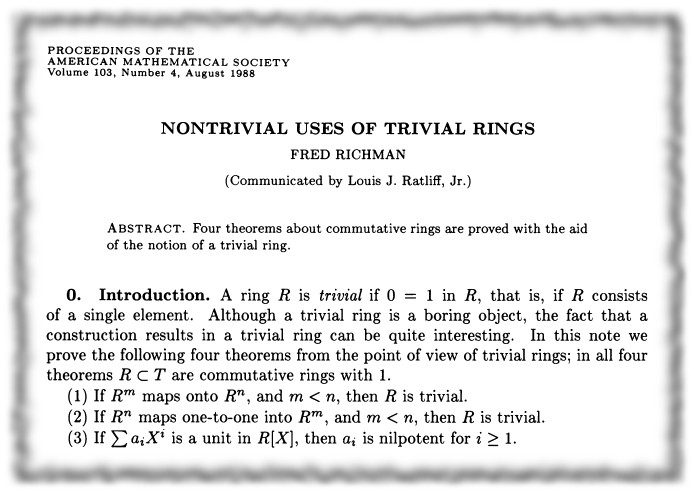
\includegraphics[width=0.8\textwidth]{nontrivial-uses-of-trivial-rings}
\end{frame}


\subsection[Properties]{Investigating the forcing model}

\begin{frame}{Investigating the forcing model}
  \vspace*{-1em}
  \begin{varblockextra}{\textwidth}{}{
    \hil{Examples:} being local, reduced, an integral domain.
  }
    \justifying
    Assuming the Boolean prime ideal theorem, any first-order
    formula ``$\forall \ldots \forall\_ (\cdots \Longrightarrow \cdots\!\,)$'',
    where the two subformulas may not contain~``$\Rightarrow$'' and~``$\forall$'',
    holds for~$A^\sim$ iff it holds for all stalks~$A_\ppp$.
  \end{varblockextra}
  \pause
  \begin{align*}
    \intertext{The forcing model has additional \hil{unique properties}, e.\,g.\@}
    A &\models \forall x\?A^\sim\_ \neg(\speak{$x$ inv.}) \Longrightarrow \speak{$x$ nilpotent} \\
    \intertext{which if~$A$ is reduced implies the \hil{field condition}}
    A &\models \forall x\?A^\sim\_ \neg(\speak{$x$ inv.}) \Longrightarrow x = 0
    \quad\text{and also} \\
    A &\models \forall x\?A^\sim\_ \neg\neg(x = 0) \Longrightarrow x = 0.
  \end{align*}
  \emph{Translation.} For any element~$x \in A$, if~$f = 0$ is the only element such
  that~$x$ is invertible in~$A[f^{-1}]$, then~$x = 0$.
\end{frame}


\section{Grothendieck's generic freeness}

\subsection{Statement}

\begin{frame}{Grothendieck's generic freeness}
  \small
  Let~$A$ be a reduced ring. \\
  Let~$B$ be an~$A$-algebra of finite type ($\cong A[X_1,\ldots,X_n]/\aaa$). \\
  Let~$M$ be a finitely generated~$B$-module ($\cong B^m/U$).

  \vspace{-1em}
  \begin{varblock}{\textwidth}{}
    \hil{Theorem.} If~$1 \neq 0$ in~$A$, there exists $f \neq 0$ in $A$ such that
    \vspace*{-0.5em}
    \begin{enumerate}
      \item $B[f^{-1}]$ and $M[f^{-1}]$ are free modules over $A[f^{-1}]$,
      \item \vspace*{-0.2cm}$A[f^{-1}] \to B[f^{-1}]$ is of finite presentation, and
      \item \vspace*{-0.2cm}$M[f^{-1}]$ is finitely presented as a module over~$B[f^{-1}]$.
    \end{enumerate}
  \end{varblock}

  \begin{columns}[t]
    \begin{column}{0.34\textwidth}
      \centering
      \ \\[0.5em]
      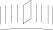
\includegraphics[width=0.7\textwidth]{generic-freeness}

      \small
      $A = k[X]$, \\ $B = M = k[X,Y]/(XY)$
    \end{column}

    \pause

    \begin{column}{0.68\textwidth}
      \vspace*{-0.5em}
      \begin{itemize}
        \item No generalization to unreduced rings.
        \item \vspace*{-0.2cm}Implies the law of excluded middle.
        \pause
        \item \vspace*{-0.2cm}\hil{Constructive restatement.} \\ If zero is the only
        element~$f \in A$ such that
        {\!\renewcommand{\insertenumlabel}{1}\usebeamertemplate{enumerate item}},
        {\!\renewcommand{\insertenumlabel}{2}\usebeamertemplate{enumerate item}}, and
        {\!\renewcommand{\insertenumlabel}{3}\usebeamertemplate{enumerate item}},
        then~$1 = 0 \in A$.
      \end{itemize}
    \end{column}
  \end{columns}
\end{frame}


\subsection{Proof}

\begin{frame}{A constructive proof}
  \small
  Let~$A$ be a reduced ring. \\
  Let~$B$ be an~$A$-algebra of finite type ($\cong A[X_1,\ldots,X_n]/\aaa$). \\
  Let~$M$ be a finitely generated~$B$-module ($\cong B^m/U$).

  \only<1>{\vspace{-1em}
  \begin{varblock}{\textwidth}{}
    \hil{Theorem.} If zero is the only element~$f \in A$ such that
    \vspace*{-0.5em}
    \begin{enumerate}
      \item $B[f^{-1}]$ and $M[f^{-1}]$ are free modules over $A[f^{-1}]$,
      \item \vspace*{-0.2cm}$A[f^{-1}] \to B[f^{-1}]$ is of finite presentation, and
      \item \vspace*{-0.2cm}$M[f^{-1}]$ is finitely presented as a module over~$B[f^{-1}]$,
    \end{enumerate}
    \vspace*{-0.5em}
    then~$1 = 0 \in A$.
  \end{varblock}}

  \emph{Constructive proof.} Observe that the theorem amounts to
  \vspace*{-0.5em}
  \begin{multline*}A \models \ulcorner\text{It's \hil{not not} the case that} \\
    \begin{minipage}{9cm}\vspace*{-0.2cm}\begin{enumerate}
      \item $B^\sim$ and $M^\sim$ are free modules over $A^\sim$,
      \item \vspace*{-0.3cm}$A^\sim \to B^\sim$ is of finite presentation, and
      \item \vspace*{-0.3cm}$M^\sim$ is finitely presented as a module
      over~$B^\sim$$\urcorner$.
    \end{enumerate}\end{minipage}\end{multline*}
  \pause
  \justifying
  Claims~{\!\renewcommand{\insertenumlabel}{2}\usebeamertemplate{enumerate item}}
  and~{\!\renewcommand{\insertenumlabel}{3}\usebeamertemplate{enumerate item}}
  follow from the fact that~$A^\sim$ is \hil{anonymously Noetherian} (any ideal
  is \hil{not not} finitely generated) which entails
  that~$A^\sim[X_1,\ldots,X_n]$ is anonymously Noetherian.

  Claim~{\!\renewcommand{\insertenumlabel}{1}\usebeamertemplate{enumerate item}}
  follows from a careful rendition of the standard linear algebra proof,
  employing Dickson's lemma to ensure termination. \qed
\end{frame}

\backupstart

\begin{frame}
  Assume that~$B^\sim$ is generated by~$(x^i y^j)_{i,j\geq0}$ as an~$A^\sim$-module.
  It's \hil{not not} the case that either some generator can be expressed as a
  linear combination of others with smaller index, or not.

  \centering
  \begin{tikzpicture}[scale=0.4]
    \begin{scope}
      \draw[step=1cm,gray,very thin] (0,0) grid (8,8);

      \draw
        (0,8) -- (0,0) -- (8,0);

      \fill[fill=blue!40!white,opacity=0.5]
        (0,8) -- (0,0) -- (6,0) -- (6,5) -- (5,5) -- (5,8);

      \fill[fill=red!40!white,opacity=0.5]
        (5,5) -- (6,5) -- (6,6) -- (5,6);

      \node[shape=circle,draw,inner sep=2pt] at (1,1) {1};
    \end{scope}

    \begin{scope}[xshift=9cm]
      \draw[step=1cm,gray,very thin] (0,0) grid (8,8);

      \draw
        (0,8) -- (0,0) -- (8,0);

      \fill[pattern=north east lines,pattern color=gray,opacity=0.5]
        (5,8) -- (5,5) -- (8,5) -- (8,8);
      \draw
        (5,8) -- (5,5) -- (8,5);

      \fill[fill=blue!40!white,opacity=0.5]
        (0,8) -- (0,0) -- (3,0) -- (3,5) -- (2,5) -- (2,8);

      \fill[fill=red!40!white,opacity=0.5]
        (2,5) -- (3,5) -- (3,6) -- (2,6);

      \node[shape=circle,draw,inner sep=2pt] at (1,1) {2};
    \end{scope}

    \begin{scope}[xshift=18cm]
      \draw[step=1cm,gray,very thin] (0,0) grid (8,8);

      \draw
        (0,8) -- (0,0) -- (8,0);

      \fill[pattern=north east lines,pattern color=gray,opacity=0.5]
        (2,8) -- (2,5) -- (8,5) -- (8,8);
      \draw
        (2,8) -- (2,5) -- (8,5);

      \fill[fill=blue!40!white,opacity=0.5]
        (0,8) -- (0,0) -- (7,0) -- (7,2) -- (6,2) -- (6,5) -- (2,5) -- (2,8);

      \fill[fill=red!40!white,opacity=0.5]
        (6,2) -- (7,2) -- (7,3) -- (6,3);

      \node[shape=circle,draw,inner sep=2pt] at (1,1) {3};
    \end{scope}

    \begin{scope}[yshift=-9cm]
      \draw[step=1cm,gray,very thin] (0,0) grid (8,8);

      \draw
        (0,8) -- (0,0) -- (8,0);

      \fill[pattern=north east lines,pattern color=gray,opacity=0.5]
        (2,8) -- (2,5) -- (6,5) -- (6,2) -- (8,2) -- (8,8);
      \draw
        (2,8) -- (2,5) -- (6,5) -- (6,2) -- (8,2);

      \fill[fill=blue!40!white,opacity=0.5]
        (0,8) -- (0,0) -- (6,0) -- (6,3) -- (5,3) -- (5,5) -- (2,5) -- (2,8);

      \fill[fill=red!40!white,opacity=0.5]
        (5,3) -- (6,3) -- (6,4) -- (5,4);

      \node[shape=circle,draw,inner sep=2pt] at (1,1) {4};
    \end{scope}

    \begin{scope}[yshift=-9cm,xshift=9cm]
      \draw[step=1cm,gray,very thin] (0,0) grid (8,8);

      \draw
        (2,8) -- (2,5) -- (5,5) -- (5,3) -- (6,3) -- (6,2) -- (8,2);

      \draw
        (0,8) -- (0,0) -- (8,0);

      \fill[pattern=north east lines,pattern color=gray,opacity=0.5]
        (2,8) -- (2,5) -- (5,5) -- (5,3) -- (6,3) -- (6,2) -- (8,2) -- (8,8);

      \fill[fill=blue!40!white,opacity=0.5]
        (0,8) -- (0,0) -- (4,0) -- (4,3) -- (3,3) -- (3,5) -- (2,5) -- (2,8);

      \fill[fill=red!40!white,opacity=0.5]
        (3,3) -- (4,3) -- (4,4) -- (3,4);

      \node[shape=circle,draw,inner sep=2pt] at (1,1) {5};
    \end{scope}

    \begin{scope}[yshift=-9cm,xshift=18cm]
      \draw[step=1cm,gray,very thin] (0,0) grid (8,8);

      \draw
        (0,8) -- (0,0) -- (8,0);

      \fill[pattern=north east lines,pattern color=gray,opacity=0.5]
        (2,8) -- (2,5) -- (3,5) -- (3,3) -- (6,3) -- (6,2) -- (8,2) -- (8,8);
      \draw
        (2,8) -- (2,5) -- (3,5) -- (3,3) -- (6,3) -- (6,2) -- (8,2);

      \node[shape=circle,draw,inner sep=2pt] at (1,1) {6};
    \end{scope}
  \end{tikzpicture}
  \par
\end{frame}

\begin{frame}{An explicit constructive proof}
  \justifying\small\fontsize{10pt}{12.3}\selectfont
  \vspace*{-0.5em}

  \hil{Lemma.} Let~$A$ be a ring. Let~$M$ be an~$A$-module with generating
  family~$(x_1,\ldots,x_n)$. Assume that the only element~$g \in A$ such that one of
  the~$x_i$ is an~$A[g^{-1}]$-linear combination in~$A[g^{-1}]$ of the other generators
  is~$g = 0$. Then~$M$ is free with~$(x_1,\ldots,x_n)$ as a basis.

  \emph{Proof.} Let~$\textstyle\sum_i a_i x_i = 0$. Let $i$ be arbitrary. In $M[a_i^{-1}]$,
  the generator~$x_i$ is a linear combination of the other generators.
  Thus~$a_i = 0$. \qed

  \hil{Theorem.} Let~$A$ be a reduced ring. Let~$M$ be a finitely
  generated~$A$-module. If zero is the only element~$f \in A$ such
  that~$M[f^{-1}]$ is finite free as an~$A[f^{-1}]$-module, then~$1 = 0$
  in~$A$.

  \emph{Proof.}
  By induction on the length~$n$ of a generating family
  $(x_1,\ldots,x_n)$ of~$M$.

  % Note that we'll apply the induction hypothesis not to the ring~$A$, but to
  % some localizations of~$A$.
  We verify the assumption of the lemma.
  Thus let~$g \in A$ be given such that one of the~$x_i$ is an
  $A[g^{-1}]$-linear combination of the others in~$M[g^{-1}]$. Therefore the
  $A[g^{-1}]$-module~$M[g^{-1}]$ can be generated by $n-1$ elements. By the
  induction hypothesis (applied to~$A[g^{-1}]$ and its
  module~$M[g^{-1}]$) it follows that $A[g^{-1}] = 0$. Therefore $g = 0$.

  Thus~$M$ is free. We finish by using the assumption for $f = 1$.
  \qed
\end{frame}

\begin{frame}{An explicit constructive proof}
  \justifying\small
  \hil{Theorem.} Let~$A$ be a reduced ring. Let~$B$ be a finitely
  generated~$A$-algebra. If zero is the only element~$f \in A$ such
  that~$B[f^{-1}]$ is finitely presented as an~$A[f^{-1}]$-algebra, then~$1 =
  0$ in~$A$.

  \emph{Proof.} Write~$B = A[X_1,\ldots,X_n]/\aaa$. We describe only the
  case~$n = 0$.

  As a first step, we verify~$\aaa = (0)$. Let~$f \in \aaa$. Then~$B[f^{-1}] =
  0$. Thus~$f = 0$ by assumption.

  We now use the assumption again, this time for~$f = 1$.
  \qed
\end{frame}

\backupend

\end{document}
